% 中文版：需要 xelatex（xeCJK）。  python main.py report 会一起编译。
\documentclass{article}
\usepackage{iclr2025_conference,times}
\usepackage{amsmath,amssymb}
\usepackage{booktabs}
\usepackage{graphicx}
\usepackage{url}
\usepackage{xcolor}
\usepackage{xeCJK}
\setCJKmainfont{Noto Serif CJK SC}
\setCJKsansfont{Noto Sans CJK SC}
\setCJKmonofont{Noto Sans Mono CJK SC}
\usepackage[colorlinks=true,linkcolor=black,citecolor=black,urlcolor=blue!60!black]{hyperref}

\graphicspath{{../results/}}

\newcommand{\shrink}{\mathrm{shrink}}
\newcommand{\trcov}{\operatorname{tr}\mathrm{Cov}}
\newcommand{\E}{\mathbb{E}}
\newcommand{\Var}{\operatorname{Var}}
\newcommand{\arm}[1]{\texttt{#1}}

\iclrfinalcopy

\title{GRPO 的收缩基线：James--Stein 何时塌缩，以及要测出差别需要什么}

\author{杨瀚文 (Hanwen Yang)\\
\texttt{hanwenya150@gmail.com}\\
代码与日志：\url{https://github.com/hyang150/GRPO_JS_Eva}
}

\begin{document}
\maketitle

\begin{abstract}
GRPO 只用同一个 prompt 采出的 $N$ 条回答来估计该 prompt 的基线，$N$ 小时这个
均值噪声很大。给定的规范提出用 James--Stein 估计量把每个组均值向 batch 均值
收缩，其收缩常数由"每样本奖励方差为 1"的假设固定。我们实现了该规范，把五个
对照基线放进同一个注册表，并在 Qwen2.5-0.5B-Instruct / GSM8K 上测量。三个结
果。(i) 直接作用于原始 $0/1$ 奖励时，规范指定的估计量塌缩成全局 batch 均值：
它假设的方差至少高估真实方差 $4$ 倍，塌缩随 prompt 数 $K$ 单调加剧，且在
$N=2$ 时对一切 $K>6$ 是一个代数恒等式。三个种子的训练中，它在 100\% 的步上
丢弃了组结构。(ii) 满足规范自己的 $\sigma^2\approx1$ 前提后，Stein 的行为得到
恢复：收缩因子与闭式解 $N\tau^2/(1+N\tau^2)$ 相差不超过 $0.02$，基线的均方误
差在仿真中下降 16--54\%。(iii) 以上任何一点在这个规模下都无法体现为端到端精
度。在 $K=32,N=2$ 下两条可证明为同一算法的臂，三个种子分别相差 $0.5$、$6.5$、
$1.5$ 个点，而文献报告的效应是 $0.65$--$1.5$ 个点；逐步梯度噪声/信号比对所有
基线都在 58--182。早先草稿报告为显著的配对梯度方差测量，因发现投影 bug 和
off-policy 采样器而撤回，且受时间限制未重做。我们还证明，规范中可选的"除以组
内标准差"在任何收缩基线下都会把退化组的优势放大 $10^4$ 倍。
\end{abstract}

\section{引言}

Group Relative Policy Optimization~\citep{shao2024deepseekmath} 把
PPO~\citep{schulman2017ppo} 的 critic 去掉，改为对每个 prompt 采样 $N$ 条回答，
用它们的平均奖励做基线。在可验证的 $0/1$ 奖励和小 $N$ 下，这个基线很粗糙：
$N=2$ 时它只有三个取值，而全对或全错的组根本没有信号。本工作拿到的规范
（\texttt{GRPO.md}，见附录~\ref{app:spec}）给出一个来自经典统计的补救：把一个
batch 里的 $K$ 个组均值看作 $K$ 个共同已知方差 $V=1/N$ 的正态均值，用正部
James--Stein 估计量~\citep{james1961} 向全局均值收缩。Stein 的结果保证总均方误
差更低，规范由此推出优势方差更低、训练更稳、可以支持更小的 $N$。

我们把这条推理链从头到尾检验了一遍。贡献如下：

\begin{itemize}\itemsep2pt
\item 六个基线的注册表（第~\ref{sec:estimators} 节），规范的逐字转录与实现
      在 $10^{-12}$ 内一致，一个到 verl 优势估计器接口的适配器，162 个测试。
      规范自带的伪代码在它的文字声称能处理的两个边界情形上崩溃
      （附录~\ref{app:conformance}）。
\item 对规范估计量何时退化为全局均值的分析（第~\ref{sec:analysis} 节）：收缩项
      的大 $K$ 极限、$N=2$ 恒等式，以及前提满足时收缩因子遵循的闭式解。
\item 真值已知的仿真（第~\ref{sec:synthetic} 节）和 $K\cdot N=64$ 的两种组形
      状、三个种子的 GRPO 训练（第~\ref{sec:training} 节），其中包含一对同算法
      复制实验，直接测出了该协议的噪声底。
\item 一份修正记录（附录~\ref{app:corrections}）：off-policy 采样器、补全
      mask 缺陷和梯度投影 bug，都在复查中发现、都已修复，并撤回被它们污染
      的结果。
\end{itemize}

主要结论在两个意义上是否定的。规范按原样写法在 $0/1$ 奖励上不工作；修正后
的版本虽然对基线做到了 Stein 定理所说的事，但没有产生这个规模的实验能分辨
的精度效应。

\section{背景}

\paragraph{GRPO。} 对 prompt $x$，策略采样 $N$ 条回答 $y_1,\dots,y_N$，得到奖励
$r_i$。GRPO 构造逐样本优势 $A_i=r_i-b$，$b$ 为组均值，可选地再除以组内标准差，
然后套用 PPO 的裁剪目标并对参考策略加 KL 惩罚。减去一个不依赖于样本的基线不
改变策略梯度的期望但降低其方差；组均值是价值函数的逐 prompt 蒙特卡洛估计，
这正是 GRPO 不需要 critic 的原因。它并不独立于 $r_i$（它包含 $r_i$），但对普通
均值而言这只是把梯度乘以 $(1-1/N)$；RLOO~\citep{ahmadian2024rloo} 的留一均值把
这一点也去掉了。

\paragraph{规范。} 记组均值 $X_k=\frac1N\sum_i r_i^{(k)}$，全局均值 $\bar X$，
$S=\sum_k(X_k-\bar X)^2$，$c=V(K-3)$，
\begin{equation}
\tilde\mu_k=\bar X+\shrink\cdot(X_k-\bar X),\qquad
\shrink=\max\!\left(0,\;1-\frac{c}{S}\right),
\label{eq:js}
\end{equation}
优势为 $A_i^{(k)}=r_i^{(k)}-\tilde\mu_k$。规范取 $V=1/N$，这在每样本奖励方差
$\sigma^2=1$ 时是正确的，并在理论部分说明奖励应先缩放到满足该条件。它的伪代
码直接使用原始奖励矩阵。

\section{分析}
\label{sec:analysis}

\subsection{前提，以及 $K$ 是什么}

GSM8K 的奖励是二值的，所以 $\sigma_k^2=p_k(1-p_k)\le\tfrac14$：比假设的至少小
$4$ 倍，跨 prompt 异方差，且对全对或全错的组恰好为零（我们的运行中 $N=8$ 时占
25--28\% 的组，$N=2$ 时占 68--70\%）。高估 $V$ 就高估 $c$，把 $\shrink$ 推向零。

$K$ 是计算优势时手头有奖励的 prompt 数，即 rollout batch，而不是反向传播的
micro-batch。Stein 现象在收缩中心固定时需要 $K\ge3$，中心为估计出的全局均值时
需要 $K\ge4$，所以常数里是 $K-3$。本工作跑 $K=8$ 和 $32$；
\citet{zeng2025shrinking} 用 64；生产训练通常是几百到几千。

\subsection{大 $K$ 极限}

由 $\E[S]\approx(K-1)\Var(X_k)$ 与 $c=V(K-3)$，记 $\tau^2$ 为各 prompt 真实通
过率的方差，
\begin{equation}
\frac{c}{S}\;\xrightarrow[K\to\infty]{}\;
\frac{V_{\text{assumed}}}{\Var(X_k)}
=\frac{V_{\text{assumed}}}{\tau^2+\sigma^2/N},
\label{eq:limit}
\end{equation}
是一个常数。$K$ 不会让收缩更强，只会让 $S$ 的噪声更小，于是估计量收敛到这个
比值决定的行为。

\textbf{如果前提成立}，$V_{\text{assumed}}=1/N$ 是精确的，极限为
$1/(1+N\tau^2)<1$，对任何 $N$ 与 $\tau^2$ 都成立：截断永远不触发，且
\begin{equation}
\shrink\;\xrightarrow[K\to\infty]{}\;\frac{N\tau^2}{1+N\tau^2},
\label{eq:eb}
\end{equation}
即经验贝叶斯后验权重——温和的收缩，随 $N$ 增大或 prompt 间差异变大而减弱。

\textbf{如果前提不成立}，如 $0/1$ 奖励，该比值至少为 $(1/N)/(\tau^2+1/(4N))$。
对第~\ref{sec:synthetic} 节使用的奖励分布，它在 $N=8$ 时为 $1.69$，$N=2$ 时为
$3.57$。超过 $1$ 时正部截断触发，估计量\emph{就是}全局均值。更大的 $K$ 让这一
点从偶然变成必然：规范指定的方法随 batch 中 prompt 增多而变差，而这正是
GRPO 的部署 regime。

\subsection{$N=2$ 恒等式}
\label{sec:identity}

$0/1$ 奖励的组均值落在 $[0,1]$，因此对任何 $K$ 有 $S\le K/4$。当 $c=(K-3)/N$
时，只要 $(K-3)/N>K/4$，即 $K>3/(1-N/4)$，截断必然触发：$N=2$ 时 $K>6$，
$N=3$ 时 $K>12$，$N\ge4$ 时不再有保证，那时需要 $S$ 足够小，而这由
式~\eqref{eq:limit} 随 $K$ 增大提供。于是在规范所针对的 $N=2$ regime 下，规范
指定的估计量对任何多于六个 prompt 的 batch 都等于全局均值，与奖励取值无关。
第~\ref{sec:floor} 节把这一点变成了一个测量。

\subsection{即便前提成立也不能迁移的东西}

三件事。Bernoulli 奖励是异方差的，所以"共同已知的 $V$"只是靠合并得到的近似；
逐组标准差不可用，因为三分之一到三分之二的组标准差为零。收缩后的基线通过
$\bar X$ 和 $S$ 依赖 $r_i$ 本身，所以策略梯度有偏——不是普通 GRPO 那种常数
因子 $(1-1/N)$，而是非线性的；只有留一构造能保持无偏。退化组按设计得到非零
优势，把全对的 prompt 往上推、全错的往下推，方向取决于 batch 碰巧偏向哪边：
这是拿噪声换偏差，不是凭空造出信号。

\subsection{标准差选项}
\label{sec:footgun}

规范提供"之后再除以组内标准差"作为可选项。普通 GRPO 在退化组上这样做是安全
的，仅仅因为那里优势恰好为零，$0/(0+10^{-4})=0$。任何收缩基线都会给这样的组
非零优势——这正是方法的意图——于是同一个表达式把它乘以 $10^4$。在 GSM8K
$K=8$、$N=8$、38\% 退化组下实测：$\Var(A)=1.07\times10^5$，梯度范数
$1.7\times10^3$；对零离散度的组不缩放则为 $0.57$ 和 $1.2$。下面所有实验都不做
标准差缩放，这也是 Dr.GRPO~\citep{liu2025drgrpo} 从另一个角度主张的选择。

\section{估计量}
\label{sec:estimators}

\begin{table}[t]\centering\small
\begin{tabular}{llp{6.4cm}}
\toprule
名称 & 基线 $b[k,i]$ & 角色 \\
\midrule
\arm{vanilla}   & 组均值                          & GRPO，现任方法 \\
\arm{rloo}      & 留一组均值                      & 无偏的方差缩减对照 \\
\arm{global}    & batch 均值                      & \textbf{消融}：过度收缩退化到的极限 \\
\arm{js\_fixed} & 式~\eqref{eq:js}，$V=1/N$        & 规范原样 \\
\arm{js\_pooled}& 式~\eqref{eq:js}，$V$ 由数据估计 & 规范作用于 $r/\sigma_{\text{pooled}}$ 后缩放回来 \\
\arm{js\_loo}   & 两级留一收缩                    & \citet{zeng2025shrinking} \\
\bottomrule
\end{tabular}
\caption{基线。没有 \arm{global} 这个对照，比较无法解释："James--Stein 有效"
和"任何非组均值的基线都有效"分不开。}
\label{tab:arms}
\end{table}

表~\ref{tab:arms} 列出六个基线。\arm{js\_pooled} 是把奖励除以合并组内标准差
$\sqrt{\operatorname{mean}_k s_k^2}$ 后套用规范的十步，再缩放回去；这一恒等关
系由测试固定在 $3\times10^{-16}$ 以内。我们把它读作"满足了自身前提的规范"，
而不是另一个方法。\arm{js\_loo} 遵循 \citet{zeng2025shrinking} 第 3.3 节的式
10 与 13--16，组均值和收缩目标都是留一的。注册表仿照 verl 的优势估计器接口，
任何一臂都能通过一个薄适配器放进该框架。训练循环把一切可能混淆基线比较的
东西固定住：无 KL 项（$\beta=0$，不加载参考模型）、不做标准差缩放、常数损失
归一化使补全长度不会重新加权更新。

\section{实验}

\subsection{真值已知的仿真}
\label{sec:synthetic}

GSM8K 上没有真值，因此基线的误差在仿真中测量：$p_k\sim\mathrm{Beta}(1.2,2.2)$
（均值 $0.35$，与模型观察到的逐 prompt 分布相符；$\tau^2/\sigma^2=0.294$），
奖励 $\sim\mathrm{Bernoulli}(p_k)$，$K=32$ 时 2000 次试验，$K$ 扫描中每个 $K$
3000 次。

\begin{table}[t]\centering\small
\begin{tabular}{rrrrrrr}
\toprule
$N$ & 退化组 & \arm{global} & \arm{js\_fixed} & \arm{js\_pooled} & \arm{js\_loo} & \arm{js\_pooled} $\shrink$（式~\ref{eq:eb}） \\
\midrule
2  & 64.5\% & $-39.6\%$  & $-39.6\%$  & $-54.4\%$ & $-51.3\%$ & 0.386 (0.370) \\
4  & 36.7\% & $+17.2\%$  & $+17.2\%$  & $-40.8\%$ & $-40.0\%$ & 0.547 (0.541) \\
8  & 18.7\% & $+131.1\%$ & $+131.0\%$ & $-26.7\%$ & $-27.0\%$ & 0.705 (0.702) \\
16 & 8.9\%  & $+355.5\%$ & $+258.8\%$ & $-15.8\%$ & $-16.0\%$ & 0.827 (0.825) \\
\bottomrule
\end{tabular}
\caption{基线相对真实 $p_k$ 的 MSE，以 \arm{vanilla} 为基准的相对值，$K=32$。
\arm{rloo} 与 \arm{vanilla} 完全相同：留一改变的是基线的独立性，不是点估计。
最后一列是 \arm{js\_pooled} 实测的收缩因子，括号内为式~\eqref{eq:eb} 的预测。}
\label{tab:synth}
\end{table}

\begin{table}[t]\centering\small
\begin{tabular}{rrrrr}
\toprule
$K$ & \arm{js\_fixed} $\shrink$ & \arm{js\_fixed} MSE & \arm{global} MSE & \arm{js\_pooled} MSE \\
\midrule
4  & 0.333 & $+1.0\%$   & $+99.1\%$  & $-9.3\%$  \\
8  & 0.058 & $+84.3\%$  & $+116.4\%$ & $-18.7\%$ \\
16 & 0.006 & $+121.7\%$ & $+125.5\%$ & $-24.4\%$ \\
32 & 0.000 & $+130.2\%$ & $+130.5\%$ & $-26.8\%$ \\
64 & 0.000 & $+133.6\%$ & $+133.6\%$ & $-28.1\%$ \\
\bottomrule
\end{tabular}
\caption{$N=8$ 下扫描 $K$。到 $K=64$ 时 \arm{js\_fixed} 与 \arm{global} 每一位
都相同。$K=4$ 时规范方法大致中性，所以小 $K$ 的实验看不出问题。}
\label{tab:ksweep}
\end{table}

表~\ref{tab:synth} 给出 $N$ 扫描。\arm{js\_fixed} 在 $N\le4$ 时就是
\arm{global}，$N=8$ 时相差不到 $0.1\%$：它完全丢弃了组结构，且 $N\ge4$ 时比普
通 GRPO 更差。估计 $V$ 修复了这一点，增益随 $N$ 减小而增大，正是方法宣称的
regime；实测收缩因子与式~\eqref{eq:eb} 相差不超过 $0.02$。表~\ref{tab:ksweep}
显示塌缩随 $K$ 单调加深，与式~\eqref{eq:limit} 的预测一致。图~\ref{fig:synth}
画出两者。

\begin{figure}[t]\centering
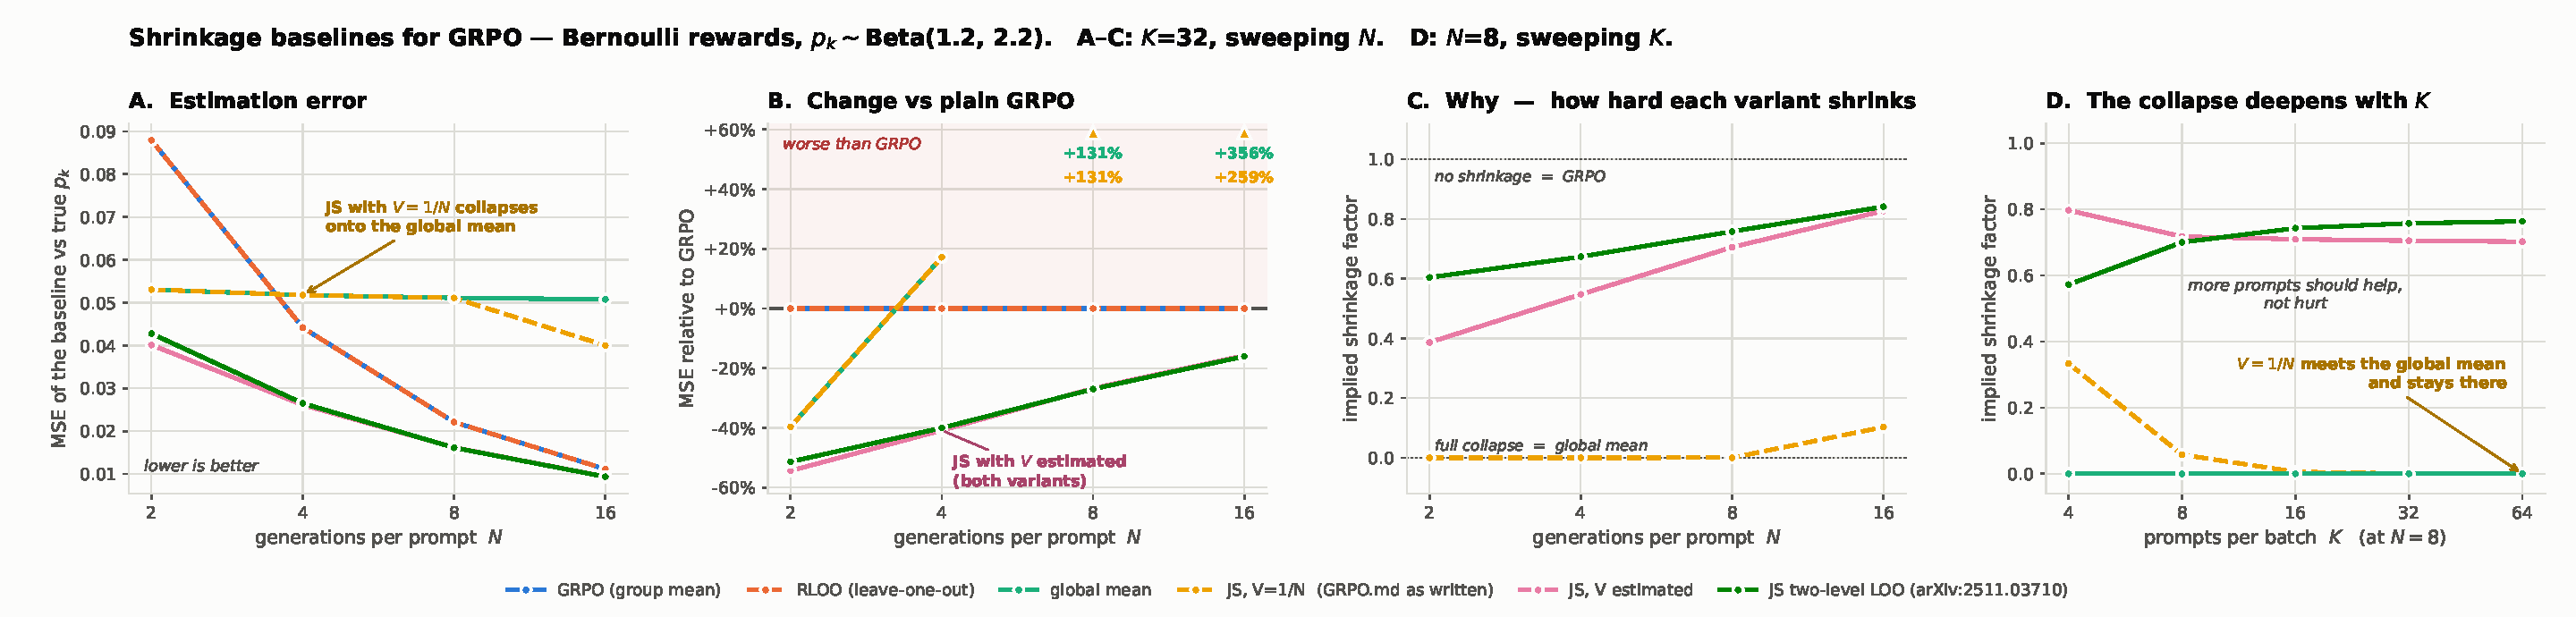
\includegraphics[width=\textwidth]{fig1_synthetic_mse.pdf}
\caption{A--C：$K=32$ 下扫描 $N$；D：$N=8$ 下扫描 $K$。\arm{js\_fixed}（虚线）
落在 \arm{global} 上；估计 $V$ 恢复了预期行为。}
\label{fig:synth}
\end{figure}

\subsection{GSM8K 上的 GRPO}

Qwen2.5-0.5B-Instruct~\citep{qwen2025} 全参微调，GSM8K~\citep{cobbe2021gsm8k}
规则正确性奖励，512 个新 token，bf16 加梯度检查点，学习率 $10^{-6}$，PPO 裁剪
$0.2$，每次 rollout 一次内层更新。开发在一张 RTX~5080 上（16\,GB；峰值
11.0\,GiB，$K{=}8,N{=}8$ 下约 25 秒一步），三种子扫描在两张 RTX~5090 上。每次
评测都按相同顺序贪心解码同样的 200 道测试题，因此 checkpoint 之间用 McNemar
检验比较，而不是看二项区间是否重叠。

两个工程细节影响数字。梯度检查点会置 \texttt{use\_cache=False}，悄悄让生成变
成长度的二次复杂度；在 rollout 前后切换它使每步时间减半。纯 bf16 在 $10^{-6}$
下会把大部分更新舍入掉——权重 $0.0145$ 的 ULP 是 $1.1\times10^{-4}$，而一步
AdamW 只移动约 $10^{-6}$；实测每步只有 $2.3\%$ 的采样权重发生变化。fp32 主权
重方案在这个 batch 下放不进 16\,GB，所以各臂共同承担 bf16 的劣势。

\subsection{三个种子，两种组形状}
\label{sec:training}

\begin{table}[t]\centering\small\setlength{\tabcolsep}{4pt}
\begin{tabular}{llrrrrrr}
\toprule
$K{\times}N$ & 臂 & 各种子最终精度 & 均值 $\pm$ sem & 对 \arm{vanilla} & $p$ & $\shrink$ & 塌缩步数 \\
\midrule
$8{\times}8$  & \arm{vanilla}    & 44.5 / 42.0 / 47.5 & $44.7\pm1.6$ & & & 1.000 & 0 \\
$8{\times}8$  & \arm{js\_pooled} & 44.0 / 45.5 / 47.0 & $45.5\pm0.9$ & $+0.8\pm1.3$ & 0.60 & 0.85 & 0--1 \\
$8{\times}8$  & \arm{js\_fixed}  & 44.0 / 47.5 / 46.0 & $45.8\pm1.0$ & $+1.2\pm2.2$ & 0.65 & 0.21 & 38--44 \\
$8{\times}8$  & \arm{global}     & 48.5 / 44.0 / 45.0 & $45.8\pm1.4$ & $+1.2\pm1.9$ & 0.61 & 0.000 & 150 \\
\midrule
$32{\times}2$ & \arm{vanilla}    & 46.0 / 45.5 / 44.5 & $45.3\pm0.4$ & & & 1.000 & 0 \\
$32{\times}2$ & \arm{js\_pooled} & 41.0 / 46.0 / 47.5 & $44.8\pm2.0$ & $-0.5\pm2.4$ & 0.85 & 0.56 & 0--1 \\
$32{\times}2$ & \arm{js\_fixed}  & 43.5 / 42.0 / 41.5 & $42.3\pm0.6$ & $-3.0\pm0.3$ & 0.009 & 0.000 & 150 \\
$32{\times}2$ & \arm{global}     & 44.0 / 48.5 / 43.0 & $45.2\pm1.7$ & $-0.2\pm1.6$ & 0.93 & 0.000 & 150 \\
\bottomrule
\end{tabular}
\caption{150 步后的最终测试精度（200 题，贪心），种子 0--2，修正后的采样器。
"对 \arm{vanilla}"为同种子内的配对差，$p$ 为自由度 2 的配对 $t$ 检验，
$\shrink$ 为隐含收缩因子的运行均值，"塌缩步数"为恰好等于 $0$ 的步数（跨种子
范围）。所有运行从同一 checkpoint 出发，因此 24 次运行第 0 步精度都是 45.0\%。}
\label{tab:phase4b}
\end{table}

两种形状各四臂，$K\cdot N=64$，每臂每步看到同样多的补全；同一种子的各臂走同
一条 prompt 流。结果见表~\ref{tab:phase4b}。

\paragraph{$K=8$、$N=8$ 下什么都分不出来。} 每臂与 \arm{vanilla} 相差不超过
$1.2$ 个点，每个 sem 都大于差值，每个 $p$ 都在 $0.6$ 左右。逐种子那一列说明
了原因：同一臂在种子之间移动 3--5 个点。只看种子 0 会得出 \arm{global} 比
\arm{vanilla} 高 $4.0$ 个点（McNemar $p=0.039$）；种子 1 和 2 分别给出 $+2.0$
和 $-2.5$。

\paragraph{$K=32$、$N=2$ 下唯一显著的那一行就是噪声底。}
\label{sec:floor}
\arm{js\_fixed} 的 $-3.0\pm0.3$（$p=0.009$）读起来像个发现。但由
第~\ref{sec:identity} 节，在这个形状下它就是 \arm{global}：三个种子全部 150 步
记录的收缩因子都是 $0$，第 1 步的记录与 \arm{global} 逐位一致，两个进程从第 2
步起才因 GPU 采样生成不可复现而分开。所以这两臂是同一算法在同种子下的三对
复制（表~\ref{tab:twins}）：它们最终相差 $0.5$、$6.5$、$1.5$ 个点。把它们当作同
一算法的六次运行合并，对 \arm{vanilla} 是 $-1.6\pm1.0$，显著性消失。自由度 2
的 $t$ 检验遇上三个碰巧落在 $0.5$ 以内的差值，可以凭空产生 $p<0.01$。

\begin{table}[t]\centering\small
\begin{tabular}{lrrr}
\toprule
种子 & \arm{global} & \arm{js\_fixed} & 差值 \\
\midrule
0 & 44.0\% & 43.5\% & $+0.5$ \\
1 & 48.5\% & 42.0\% & $+6.5$ \\
2 & 43.0\% & 41.5\% & $+1.5$ \\
\bottomrule
\end{tabular}
\caption{同一算法在每个种子下跑两次（$K=32$，$N=2$）。这个离散就是本协议的
run-to-run 项。早先在 1.1 采样器下的两次运行估计为 $3.0$ 个点。}
\label{tab:twins}
\end{table}

这一设定下文献报告的效应是 $0.65$--$1.5$ 个点（\citet{zeng2025shrinking}
表 2：同模型同任务，$N=8/4/2$ 下 JS 减 GRPO，$K=64$，500 步，五个种子）。噪声
底是效应的 2--5 倍；在这样的离散下分辨一个点的效应，每臂需要大约 20--40 个
种子。

\paragraph{扫描确实确立了什么。} 规范原样在它所针对的 $N=2$ 下，在 100\% 的步
上丢弃了组结构（$N=8$ 时为 25--30\%）；\arm{js\_pooled} 在 $N=2$ 时保留 56\%、
$N=8$ 时保留 85\%，即 Stein 结果所要求的温和收缩。"训练更稳"的说法得不到支
持：没有任何一臂裁剪过任何一步梯度，采样 token 熵对所有臂一样从 $0.52$ 降到
$0.26$--$0.33$，逐步梯度噪声/信号比（\citet{zeng2025shrinking} 式 17--18，跨
micro-batch）在 58--182，且 32--45\% 的步返回非正的信号估计。每步 8 或 32 个
prompt 时，梯度对每个基线都几乎全是噪声，这个比值分不开它们。这些步作为右删
失（$+\infty$）报告而非丢弃，丢弃会把中位数往下拉。图~\ref{fig:train} 显示两
种形状的种子 0。

\begin{figure}[t]\centering
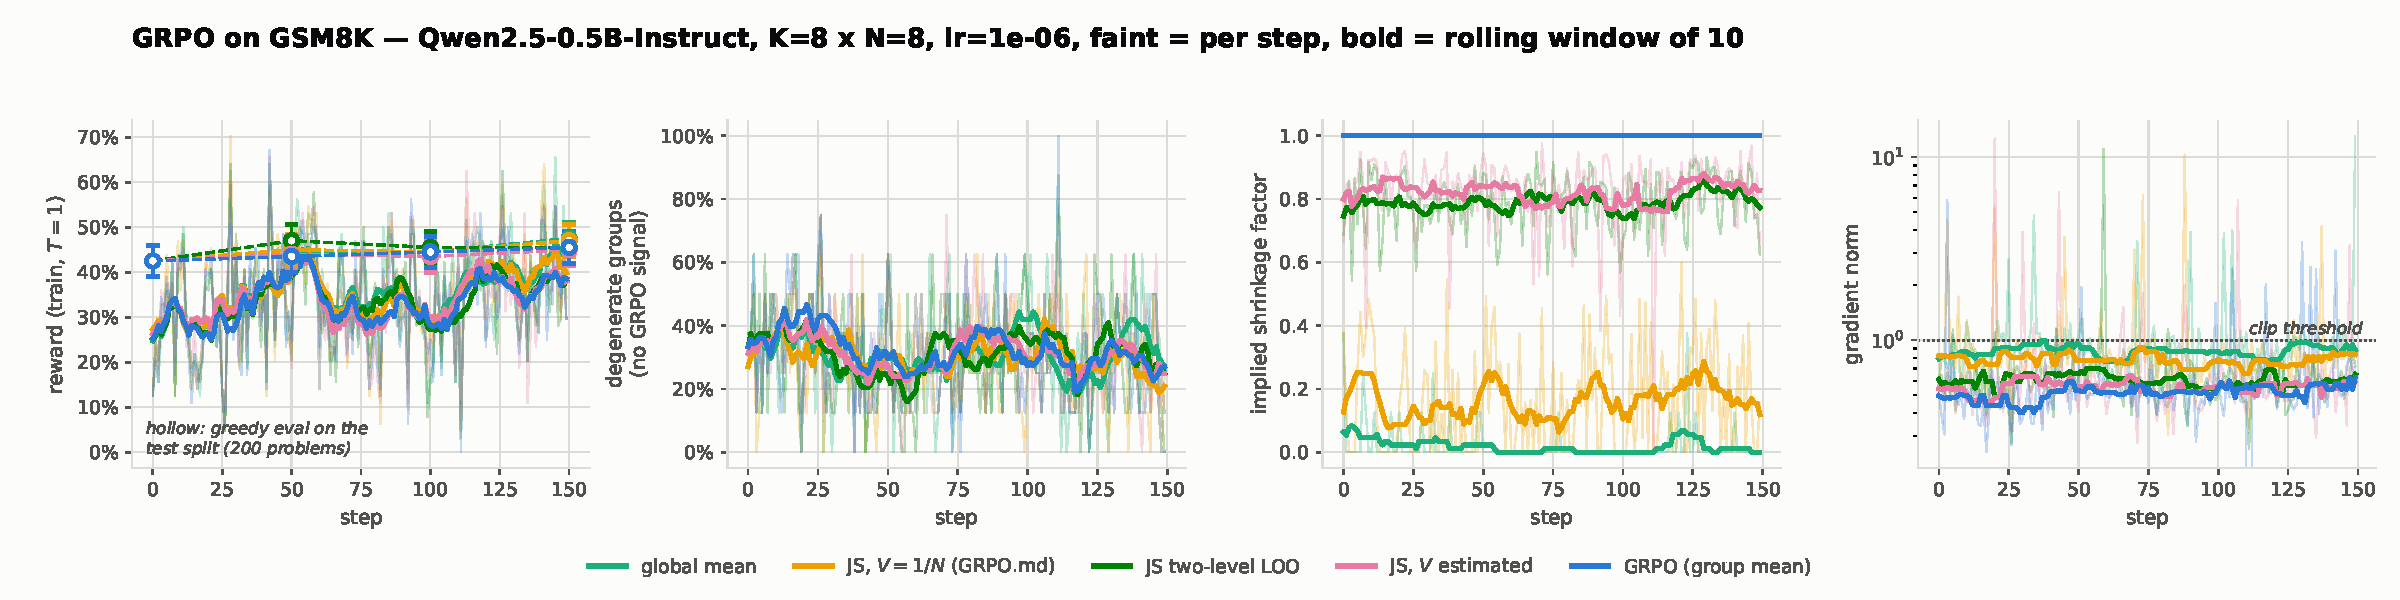
\includegraphics[width=\textwidth]{fig3_training.pdf}\\[4pt]
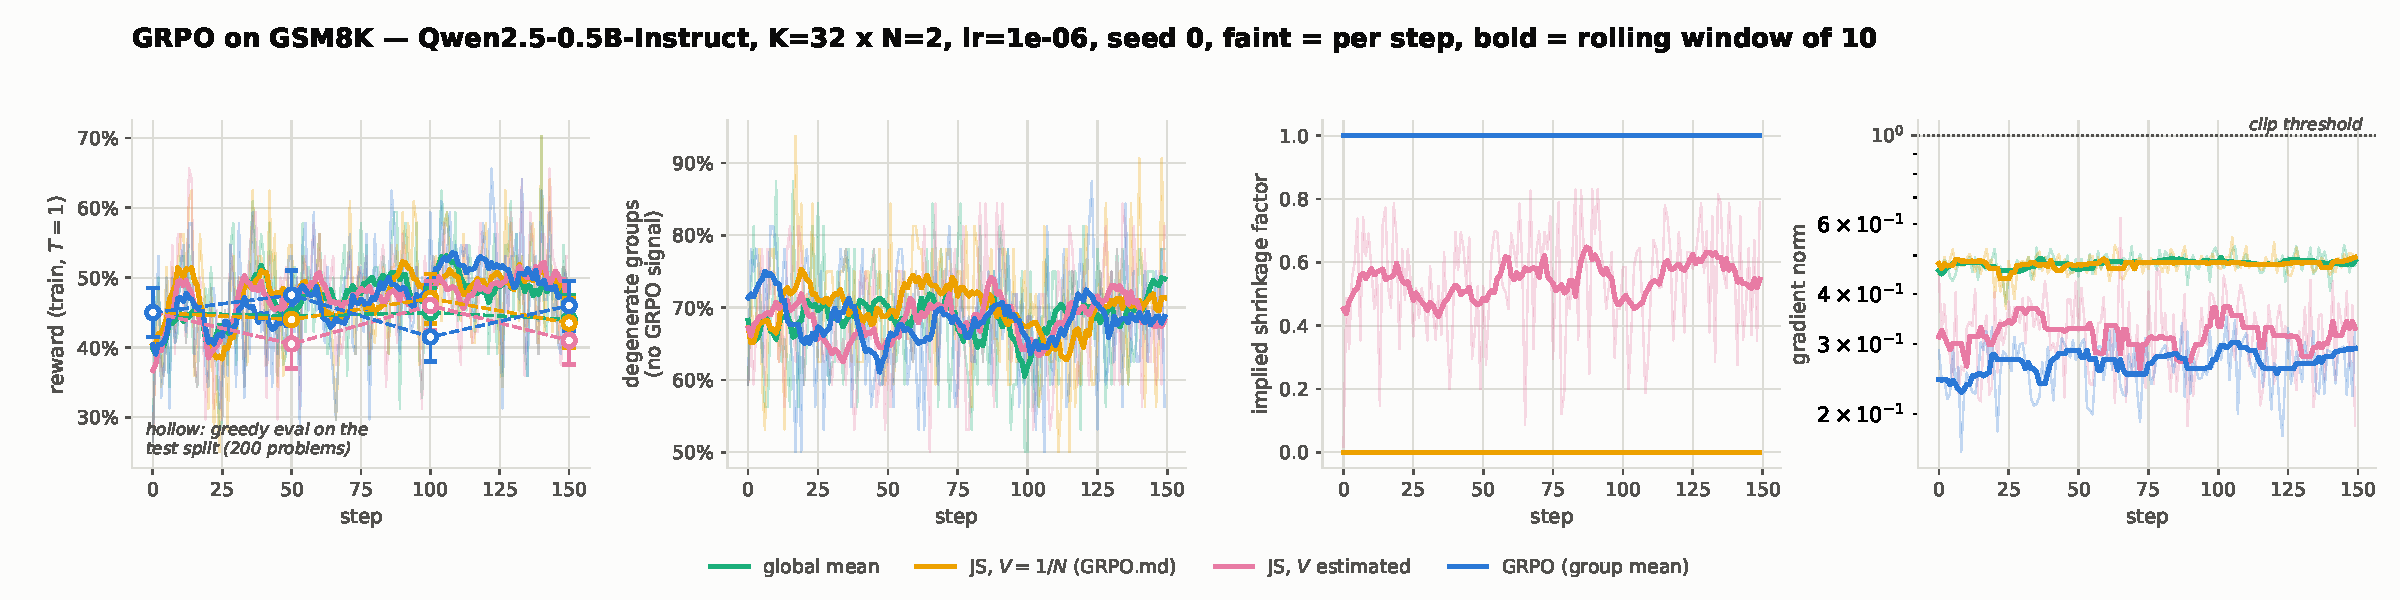
\includegraphics[width=\textwidth]{fig3_training_k32n2.pdf}
\caption{种子 0，$K{=}8,N{=}8$（上）与 $K{=}32,N{=}2$（下）。奖励和退化组两个面
板重叠；收缩面板把各臂分开，$N=2$ 时 \arm{js\_fixed} 整个运行都落在
\arm{global} 的零线上。没有任何梯度范数达到裁剪阈值。}
\label{fig:train}
\end{figure}

\subsection{一项撤回的测量}
\label{sec:gradvar}

因为训练运行分辨不了效应，早先的草稿直接测量估计量：所有基线对同一批冻结
策略的 rollout 打分，用 Hutchinson 探针估计梯度协方差的迹除以
$\lVert\E[g]\rVert^2$，在 200 个 batch 上 bootstrap。它报告 \arm{js\_loo} 相对
GRPO 为 $-21.4\%$ $[-51.5,-7.8]$。两个缺陷使其无效：探针在形状相同的参数张量
之间复用了随机数，且所有 rollout 都用 checkpoint 默认的 $1.1$ 重复惩罚采样，
而不是从策略本身采样（附录~\ref{app:corrections}）。这个仪器本身也脆弱：
$\lVert\E[g]\rVert^2$ 只占 $\E\lVert g\rVert^2$ 的 $8\%$，还是作差得到的。投影
已修复，并加入了不依赖探针的估计器——对独立的 batch，
$\E\langle g_b,g_{b'}\rangle=\lVert\E[g]\rVert^2$ 精确成立，所以不相交的 batch
对给出两个量的无偏样本——两者都在模拟梯度上通过了测试。受时间限制，这项测
量没有在模型上重做。历史表格放在附录~\ref{app:gradvar}，作为仪器的记录而非
证据。

\section{相关工作}

\citet{zeng2025shrinking} 是同一思路但把前提处理好了：组内方差和 prompt 间方
差都从 batch 估计，两层都是留一的所以策略梯度保持无偏，且没有超参数。这就是
这里的 \arm{js\_loo}。他们报告在同模型同任务、$K=64$ 下比 GRPO 高
$0.65$--$1.5$ 个点，梯度方差低 $11$--$67\%$。EBPO~\citep{han2026ebpo} 走经验贝
叶斯路线：向一个在线维护的全局先验而不是 batch 均值收缩，收缩强度由组内/组
间方差比决定。它宣称的特性——全零组仍得到非零信号——正是
第~\ref{sec:analysis} 节归为偏差的那个机制。\citet{efron1975} 把 James--Stein
用于二项比例，正是 $0/1$ 奖励的情形；他们对 $\sigma^2\ne1$ 的处理是在收缩前做
反正弦平方根方差稳定变换。我们改用合并组内标准差；那个变换是更正统的路线，
这里没有尝试。RLOO~\citep{ahmadian2024rloo} 与 Dr.GRPO~\citep{liu2025drgrpo}
分别是 \arm{rloo} 对照和"默认不缩放"的依据。

\section{局限与结论}

两种组形状各三个种子，每个精度差值都落在自己的标准误内，同算法对相差
$0.5$--$6.5$ 个点；两个方向上都不做精度声明。配对梯度方差测量是这个规模下唯
一可能分开各基线的仪器，它已撤回且未重做。\arm{rloo} 和 \arm{js\_loo} 没有进
入三种子扫描。单一模型、单一任务；塌缩阈值是否随奖励密度移动未经测试。

本工作确立的东西在其精确之处是精确的。规范指定的估计量按其伪代码作用于
$0/1$ 奖励时就是全局 batch 均值——对任何 $N$ 在 $K$ 趋于无穷时渐近成立，对
$N=2$ 在一切 $K>6$ 下恒等成立——训练日志也显示了这一点。满足规范自身的前
提后，恢复的是 Stein 定理描述的那个估计量，其收缩因子遵循经验贝叶斯闭式解。
这个估计量能否改进训练，是这个规模的实验回答不了的问题；而一个只报告单个种
子、或用自由度 2 的 $t$ 检验的协议，会把它答错。

\bibliography{refs}
\bibliographystyle{iclr2025_conference}

\appendix

\section{规范}
\label{app:spec}

\texttt{GRPO.md} 依次给出：动机（小 $N$ 的组均值噪声大）；模型
$X_k\sim\mathcal N(\mu_k,V)$，$V=1/N$，其前提是奖励已缩放到
$\sigma^2\approx1$；式~\eqref{eq:js} 的正部 James--Stein 估计量，$c=(K-3)/N$；
十个实现步骤（组均值、全局均值、$S$、$c$、$K<4$ 回退、带 $\varepsilon$ 保护的收
缩因子、$S=0$ 情形、截断、收缩后均值、优势）；一段 Python 伪代码；以及可选的
除以组内标准差。

\section{与伪代码的一致性}
\label{app:conformance}

\texttt{tests/test\_spec\_conformance.py} 转录了十个步骤，并另外逐字转录了
Python 伪代码，两者都对实现运行。在边界情形之外，伪代码与 \arm{js\_fixed} 在
连续奖励和 $0/1$ 奖励上都在 $10^{-12}$ 内一致。在它自己的边界情形上，伪代码
跑不起来：

\begin{center}\small
\begin{tabular}{lp{8.6cm}}
\toprule
输入 & 伪代码的行为 \\
\midrule
$K<4$ & \texttt{IndexError}：$\bar X$ 是 0 维张量，\texttt{unsqueeze(1)} 越界 \\
$S=0$ & \texttt{TypeError}：Python 的 \texttt{max(S, eps)} 在 $S<\varepsilon$ 时返回 float \texttt{eps}，\texttt{torch.clamp} 拒绝 float \\
$K=8$、$N=8$、$0/1$ 奖励、$S>0$ & 能运行，且等于 \arm{js\_fixed} \\
\bottomrule
\end{tabular}
\end{center}

两处偏离，均有断言。步骤 5 的文字在 $K<4$ 时返回逐组均值；伪代码修好索引后
返回的是以全局均值中心化的奖励——即 \arm{global} 臂，不再是 GRPO。我们遵循
文字。步骤 7 的"$S=0\Rightarrow$ 收缩因子为 $1$"在伪代码中不可达；我们改为截
断到 $0$，观测上等价，因为 $S=0$ 迫使 $\mathrm{diff}=0$。

\section{修正}
\label{app:corrections}

初稿后复查发现，均已在代码中修复。
\begin{enumerate}\itemsep2pt
\item \textbf{off-policy rollout（2026-09-04）。} \texttt{generate()} 设置了温
      度、top-$p$ 与 top-$k$ 但没有设置 \texttt{repetition\_penalty}，于是落到
      checkpoint 的 \texttt{generation\_config}——Qwen2.5-Instruct 为 $1.1$。
      补全从带惩罚的分布采样，而损失用的是原始策略的对数概率，每个实验的每一
      臂都如此。循环现在显式传 $1.0$。第~\ref{sec:training} 节的三种子扫描在
      修复之后运行；附录~\ref{app:seed0} 的种子 0 五臂扫描和梯度测量则不是。
\item \textbf{投影 bug（2026-09-03）。} Hutchinson 探针在形状相同的参数张量间复
      用了随机数。已修复（每个探针一条连续随机流）；回归测试把投影协方差与精
      确协方差比较。
\item \textbf{补全 mask（2026-09-04）。} 只把 \texttt{<|im\_end|>} 当作停止
      token；Qwen2.5 还会在 \texttt{<|endoftext|>} 上停止，而它同时是 pad
      token，于是这样结束的补全被当成 512 个有效 token 计分，包括 padding。
      mask 现在在所有终止符加 pad id 上停止。
\item \textbf{收缩诊断（2026-09-04）。} 均值等于全局均值的组被记为"未收缩"而不
      是"未定义"。仿真表已用修正后的诊断重新生成（\arm{global} 现在显示定义上
      的 $0$；MSE 列移动不超过 $1.5$ 个百分点）。
\end{enumerate}

\section{1.1 采样器下的种子 0 扫描}
\label{app:seed0}

第一次扫描，已被取代，留作记录：五臂，150 步，同一种子，同样的 200 道测试题。

\begin{center}\small
\begin{tabular}{lrrrrrr}
\toprule
臂 & eval@0 & eval@final & $\Delta$ & $p$ & $\shrink$ & 塌缩 \\
\midrule
\arm{vanilla}    & 42.5\% & 45.5\% & $+3.0$ & 0.24 & 1.000 & 0/150 \\
\arm{js\_pooled} & 42.5\% & 45.0\% & $+2.5$ & 0.27 & 0.850 & 1/150 \\
\arm{js\_loo}    & 42.5\% & 45.5\% & $+3.0$ & 0.21 & 0.818 & 0/150 \\
\arm{js\_fixed}  & 42.5\% & 47.0\% & $+4.5$ & 0.11 & 0.202 & 64/150 \\
\arm{global}     & 42.5\% & 47.5\% & $+5.0$ & 0.06 & 0.025 & 133/150 \\
\bottomrule
\end{tabular}
\end{center}

没有任何显著结果；五臂之间 2.5 个点的离散低于单臂对自身的噪声底。收缩列分成
精度分辨不出的几层，独立推导的 \arm{js\_pooled} 与 \arm{js\_loo} 相差不超过
$0.03$。\arm{global} 的 $0.025$ 是附录~\ref{app:corrections} 所述的诊断伪影。
这次扫描的裁剪次数（\arm{global} 150 步中 36 次，\arm{vanilla} 9 次）和熵差异
在修正后的采样器下消失。

\section{撤回的梯度测量}
\label{app:gradvar}

200 个配对 batch，$K=8\times N=8$，策略冻结，平均精度 29.1\%，1.1 采样器，有
bug 的投影。区间为以 24 个探针为条件、在 batch 上的配对 bootstrap。

\begin{center}\small
\begin{tabular}{lrrl}
\toprule
基线 & 噪声/信号 & 对 GRPO & \\
\midrule
\arm{vanilla}    & 11.5 & ---                      & \\
\arm{rloo}       & 11.5 & $-0.3\%$ $[-2.5,+6.9]$   & 仪器检查 \\
\arm{js\_loo}    & 9.1  & $-21.4\%$ $[-51.5,-7.8]$ & 撤回 \\
\arm{js\_pooled} & 9.9  & $-14.4\%$ $[-38.2,+0.8]$ & 撤回 \\
\arm{js\_fixed}  & 6.0  & $-48.1\%$ $[-81.3,-15.8]$& 有偏估计量 \\
\arm{global}     & 5.8  & $-49.7\%$ $[-83.5,-15.6]$& 有偏估计量 \\
\bottomrule
\end{tabular}
\end{center}

即便这些数字成立，\arm{js\_fixed} 和 \arm{global} 也不是"最好"：它们瞄准的是
另一个 $\E[g]$，因为给全对的组一个正优势会用一个只是把简单题往上推的分量抬
高 $\lVert\E[g]\rVert^2$。分母更大不等于信号更多。

\section{复现}

\begin{verbatim}
uv sync && python main.py smoke
python -m pytest tests/ -q          # 162 tests
python main.py synthetic --k 32 --n 2 4 8 16
python experiments/synthetic_mse.py --k 4 8 16 32 64 --n 8 \
    --trials 3000 --out results/synthetic_k_sweep.json
python main.py sweep --seeds 0 1 2 --k 32 --n 2 --track-grad-var \
    --baselines vanilla js_fixed js_pooled global
python main.py sweep --seeds 0 1 2 --k 8  --n 8 --track-grad-var \
    --baselines vanilla js_fixed js_pooled global
python main.py compare --glob 'train_*_k8n8_s*.jsonl'
python main.py compare --glob 'train_*_k32n2_s*.jsonl'
python main.py figures
\end{verbatim}

第~\ref{sec:training} 节的 24 份逐步日志已提交在 \texttt{results/} 下；它们无法
逐位复现（第~\ref{sec:floor} 节），这正是保留它们的原因。

\end{document}
